\section{Results}
  \label{sec:results}

Our technique was able to determine the worst-case time
complexity of \textit{SchemaAnalyst} with regard to the number of check
constraints on the input schema, using the
\textsc{constraintCACCoverage} coverage criterion and the
\textsc{directedRandom} data generator. Under these conditions, 
\textit{SchemaAnalyst} displayed $O(n^2)$ behavior. Figures~\ref{fig:iTrust} 
and~\ref{fig:NistWeather} show the data collected during the experiment with a
quadratic fit. The horizontal axis shows by what factor the number of initial
check constraints $i$ have been increased. For $x = 100$, the number of check
constraints on the schema is $100i$. The vertical axis shows the time in
nanoseconds \textit{SchemaAnalyst} needed to generate a test suite for
the input schema. Each point on the graph represents the amount of time
\textit{SchemaAnalyst} ran for a schema with $ix$ check constraints.
The equation shown is the best fit quadratic equation for that data.  A
quadratic relationship indicates that \textit{SchemaAnalyst} is
$O(n^2)$.  The value $r^2$ is a measure of the quality of fit between a model and
the data. The closer $r^2$ is to $1$, the better the quality of the
model.  An $r^2$ of $.997$ and $1$ indicates that the models are a good fit for
the data.

\begin{figure*}
\centering
  \centering
  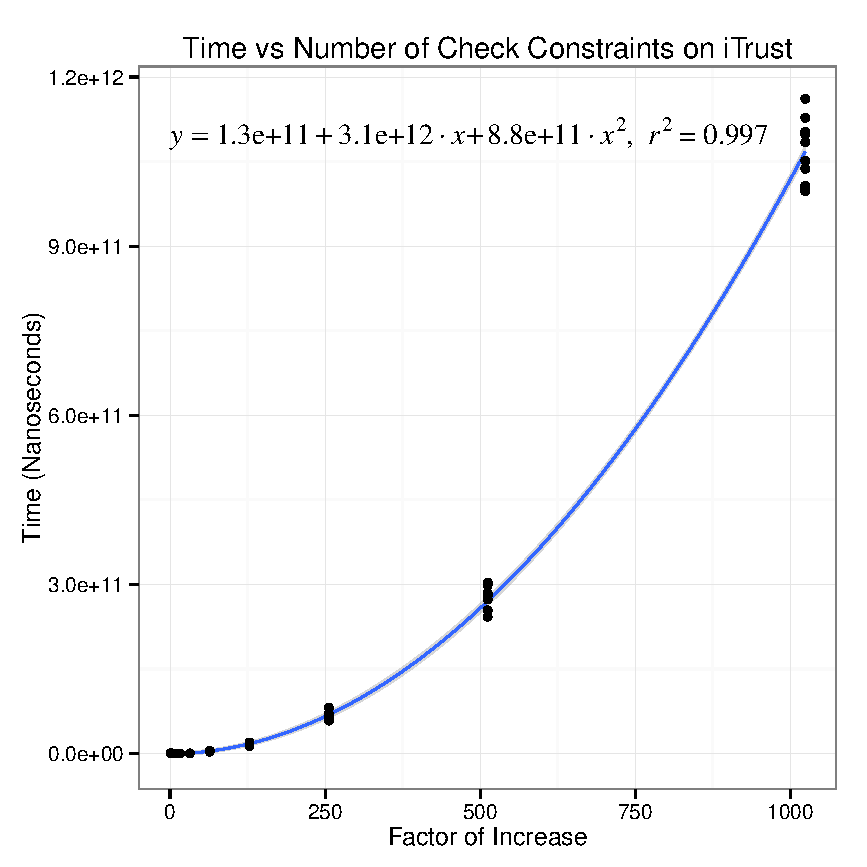
\includegraphics[width=.5\linewidth]{../results/iTrustChecks.pdf}
  \caption{Time vs Check Constraints on iTrust.}
  \label{fig:iTrust}
\end{figure*}
\begin{figure*}
  \centering
  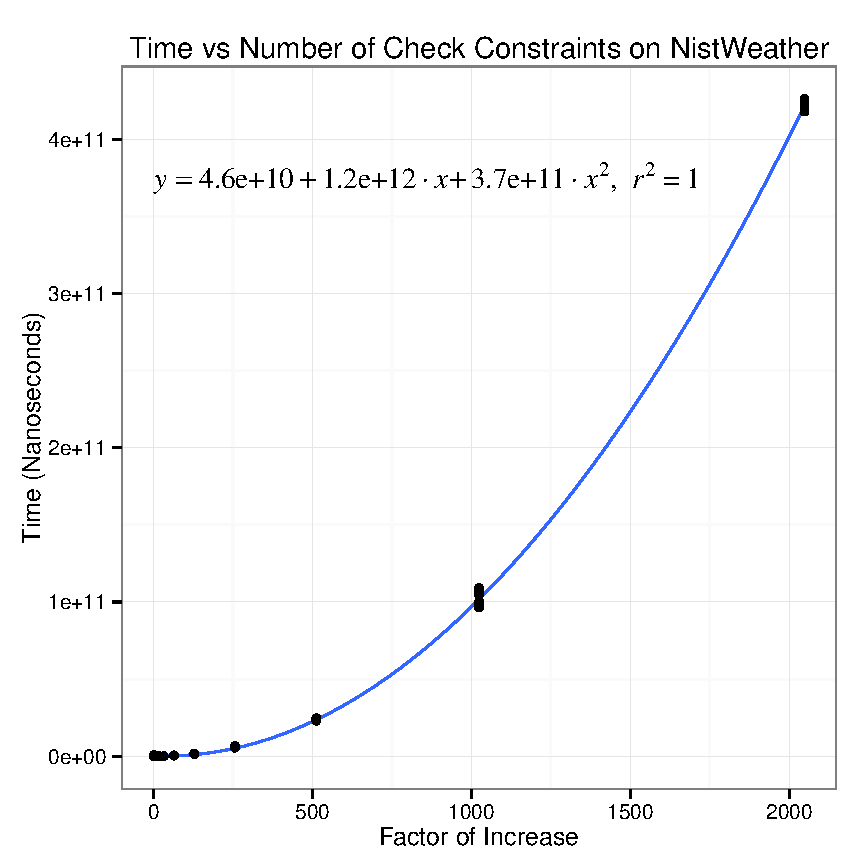
\includegraphics[width=.5\linewidth]{../results/NistWeatherChecks.pdf}
  \caption{Time vs Check Constraints on NistWeather.}
  \label{fig:NistWeather}
\end{figure*}

\subsection*{Threats to Validity}

Our technique for doubling the number of check constraints on the schema
is simply to duplicate the existing check constraints. It is possible
that \textit{SchemaAnalyst} does less work processing these copied check
constraints than it would given unique check constraints. However,
doubling the check constraints in this way is an easy to implement,
semantically significant way of evaluating \textit{SchemaAnalyst}.

Additionally, since worst-case time is only apparent for large $n$, 
it is possible that the experiment terminated too quickly.  To guard 
against this problem, Algorithms~\ref{alg:convergence} and~\ref{alg:tuning}
were tested on various other algorithms with known worst-case complexities, and 
found to be reliable.
